% Do not forget to include Introduction
%---------------------------------------------------------------
\chapter{Úvod}
% uncomment the following line to create an unnumbered chapter
%\chapter*{Introduction}\addcontentsline{toc}{chapter}{Introduction}\markboth{Introduction}{Introduction}
%---------------------------------------------------------------
\setcounter{page}{1}

Testování je nepostradatelnou částí životního cyklu vývoje softwaru. S rostoucí složitostí a velikostí systémů také roste potřeba automatizovaných testů. K tomu nám může pomoci použití různých frameworků, které přidávají mechanizmy, které testování aplikací mají zrychlit a zjednodušit. V tomto textu se zaměřím výhradně na Robot Framework, pro který byla v rámci tohoto projektu vyvinuto rozšíření, které umožňuje testování tabulkových souborů. To zahrnuje běžné formáty - .xlsx pro modrení excelové soubory, jeho starší předchůdce .xls a v neposlední řadě .csv jakožto textovou reprezentaci pro tabulkové soubory.

\section{Cíle práce}

Cílem této práce je navrhnout a implementovat open-source knihovnu pro Robot Framework, pro práci s tabulkovými soubory. Nově implementovaná knihovna umožní práci s několika typy tabulkových souborů, streaming a in-memory mód pro vybrané typy. Hlavním motivem bylo vytvořit knihovnu, která bude mít možnost spustit v módu, který šetří paměť. Návrh knihovny musí být dostatečně flexibilní pro budoucí rozvoj dalších funkcionalit, přidání dalších typů souborů a v neposlední řadě pro budoucí optimalizaci kód z hlediska použitých technologií. Výsledná implementace bude v jazyce Python, na který je Robot Framework napsaný. Jednotlivé cíle práce:

\begin{itemize}
    \item Provedení analýzy potřeb uživatelů
    \item Rešerše a analýza stávajících řešení
    \item Vytvoření návrhu a struktury knihovny
    \item Implementace knihovny podle návrhu
    \item Otestování a zdokumentování knihovny
    \item Publikace knihovny jakožto open-source
\end{itemize}

%---------------------------------------------------------------
\chapter{Analýza}
%---------------------------------------------------------------

V této kapitole se budu věnovat teoretické části bakalářské práce. Proberu návrhové vzory, architektonické principy, technologie, stávající řešení, metody testování. Veškerá probraná témata v této kapitole jsou teoretický základ pro následný návrh a implementaci knihovny 

\section{Architektura}

Jedním z prvním a zároveň tím jedním z nejduležitějších rozhodnutích ve vývoji softwaru je jeho architektura. Architektur je mnoho, všechny mají za cíl jednu hlavní věc, oddělení odpovědnosti jednotlivých částí softwaru. Tohoto oddělení docilují jednotlivé architektury pomocí rozdělení na vrstvy.

Tímto rozdělením jsme u architektur schopni docílit následujících věcí:

\begin{itemize}
    \item Škálovatelnost
    \item Testovatelnost jednotlivých částí
    \item Nezávislost na UI\footnote{User Interface}, databázi, frameworku
\end{itemize}

Software je napsán monoliticky, veškerá funkcionalita programu je zabalena na jednom místě. Dále tedy popíši možné vnitřní architektury, tedy některé z možností, jak je možné program strukturovat uvnitř jednoho projektu.\cite{Architecture} \cite{Monolitic}

\subsection{Layered architecture}

Jedna z nejběžnějších architektur pro vývoj softwaru. Jedná se o návrh, kdy se software skládá z několika na sobě posazených oddělených vrstev, které spolu komunikují. Části které spolu úzce souvisí poté většinou leží na stejné vrstvě.

Mezi charakteristiky patří to, že vrstvy zásadně komunikují pouze s vrstvami, které jsou zasazené pod nimi. Architektura také zajištuje izolaci, kdy změny v jednotlivých vrstvách by neměli mít vliv na vrstvy ostatní. Každá vrstva by měla mít jasně stanovenou odpovědnost. Rozdělení může vypadat následovně:

\begin{itemize}
    \item Prezenční vrstva, která je zodpovědna za komunikaci softwaru s uživatelem
    \item Vrstva aplikační logiky, která provádí aplikační požadavky aplikace
    \item Doménová vrstva, která se stará o algoritmy, komponenty
    \item Perzistentní vrstva, která se stará o data, komunikaci s databází
\end{itemize}

Tato architektura je jedna z nejznámějších a nejvíce používaných. Dobře se udržuje díky rozdělení na jednotlivé vrstvy, které se neovlivňují. Díky tomu je také jednoduší testování, kde jednotkové testy dobře otestují pouze funkčnost dané vrstvy, integrační zase komunikaci s nižšími vrstvami.
Mezi nevýhody patří horší škálovatelnost, kdy architektura vyžaduje hodně potřebného kódu pro napsání nové funkčnosti. Další problémem jsou vrstvy které občas mohou působit jako pouhý průtok informací (Sinkhole Anti Pattern), který vede k větší komplexitě a ztrátu efektivnosti. \cite{Layer1} \cite{Layer2}

\subsection{Hexagonal architecture}

Jinak referována také jako "Ports and Adapters".Definuje "Port" jakožto vstupní bod do aplikace, který je determinován rozhraním, přes který se s aplikací komunikuje. Zároveň porty také slouží pro komunikaci s externími systémy, jako například databáze, ostatní aplikace, systém pro zpracování zpráv. S portem se komunikuje pomocí "Adaptéru", který slouží jako prostředek pro komunikaci s aplikací skrz port. Toto vytváří abstrakci, kdy jádro aplikace je izolováno před externími nástroji a technologiemi.

Jádro aplikace obsahuje servisní a doménovou vrstvu, což jsou obě věci vyjadřující čistě aplikační logiku programu.

Tato architektura rozlišuje 2 strany komunikace:

\begin{itemize}
    \item Hlavní aktor, což je externí aktor, který iniciuje komunikaci s naší aplikací pomocí námi definovaného rozhraní
    \item Vedlejší aktor, což jsou externí systémy, které aplikace používá nebo s nimi komunikuje
\end{itemize}

Tato struktura vynucuje DIP\footnote{Dependency Inversion Principle}. Jádro aplikace určuje striktní pravidla skrz abstraktní rozhraní (Porty). Externí technologie (Adaptéry) jsou nuceny se jádru přizpůsobit, než aby toto přizpůsobení dělalo jádro oproti různým externím technologiím.

Toto způsobí, je možné vyměnit adaptéry bez jakéhokoliv zásahu do logiky jádra programu. Pro testovnání to znamená, že můžeme napsat vlastní testovací adaptér, který funkcionalitu jádra otestuje. \cite{Hexagonal}

\subsection{Mikrokernel Architecture}

Také známa jako "Plug-in", je ideální pro aplikace, u kterých chceme více rámcově hodně integrací na externí entity u kterých přesně nevíme, jak budou vypadat. Skládá se ze 2 hlavních komponent, jádro a přípojné komponenty. 

V jádru se udržuje minimální funkcionalita nutná pro běh aplikace. Při změně jádra se narozdíl od ostatních aplikací nic ve zbytku aplikace nezmění, jelikož jednotlivá pravidla a funkcionality aplikace jsou izolovány v přípojných komponentách, které jsou navzájem nazávislé.

Na správu jednotlivých nezávislých komponent slouží takzvané "registry", kde se aplikace registrují a odhlašují podle toho, kdo zrovna komunikuje s jádrem aplikace.

Smlouva (contract) definuje standartní příchozí a odchozí data mezi modulem a jednotlivými komponentami. Pokud komponenta není schopna smlouvu dodržet, je možné použít adaptér. Toto zajištuje, že jádro aplikace nikdy nemusí implementovat speciální kód pro externí komponenty. \cite{Microkernel}

\section{Principy znovupoužitelnosti}



\section{Návrhové vzory}

Návrhové vzory(Design patterns) jsou typická řešení pro běžné problémy, se kterými se v programování setkáváme. Jsou to předdělaná obecná řešení, která řeší stále dokola vyskytující se problémy při návrhu aplikací. Návrhové paterny dělíme na následující:

\begin{itemize}
    \item Creational design patterns, které slouží jakožto mechanismy pro vytváření objektů, s durázem na flexibilitu a přepoužití kódu
    \item Structual desing pattens, sloužící pro složení objektů a tříd do velkých struktur, kdy zároveň zachováváme flexibilitu a efektivnost
    \item Behavioral design patterns, zaměřující se na algoritmy a rozdělení odpovědnosti mezi objekty
\end{itemize}

Dále vysvětlím a definuji vzory, které poté budou použity v implementaci. \cite{DesignPatterns}

\subsection{Facade}

Strukturální návrhový vzor, který poskytuje jednoduchý high-level interface pro knihovny, frameworky nebo komplexní množiny tříd. Při práci s takovýmito aplikacemi často musíme spravovat mnoho různých objektů, inicializovat je ve specifickém pořadí a řešit závislosti. To vede k provázání business logiky a interními detaily implementace s externími aplikacemi, tím se stěžuje vývoj i údržba.

Tento návrhový vzor řeší problém pomocí zaobalení aplikace do jedné třídy (fasády), která bude mít jasně definované rozhraní. To je sice více limitující, než kdybychom interagovali naší aplikaci na vnitřní systém přímo, dovolí nám to ale vybrat pouze věci, které chceme vystavit externím uživatelům.

Uživatel tedy komunikuje výhradně s fasádou. Samotná aplikace přitom o fasádě vůbec neví a interně komunikuje dále meze změny. Naopak to platí stejně, při změnách v jádru aplikace uživatel nepozná změnu, jelikož je odstíněn od detailů pomocí vystaveného rozhraní. \cite{Fasade}

\subsection{Bridge}

Strukturální návrhový vzor, který nám dovoluje rozdělit velkou třídu nebo množinu sobě podobných tříd do více hierarchií, které můžou být vyvíjeny nezávisle na sobě.

Jako příklad si vezmeme geometrický objekt Shape. Shape má 2 podtřídy, Circle a Square. A tuto hierarchie chceme rozšířit o barvy, náš Shape budeme chtít Blue a Red. Pomocí klasického dědění nebudou muset vzniknout třídy 2, ale rovnou 4, BlueCircle, RedCircle, BlueSquare, RedSquare. Přidání dalších vlastností třídy Shape nám bude náročnost hierarchie růst exponencionálně. S rostoucí velikostí projektu bude udržování této architektury stále těžší a těžší.

Problém nastává, protože se snažíme Shape rozšiřovat do 2 více různých dimenzí najednou, formy a barvy. Bridge tento problém řeší změnou z dědění na kompozici objektů. Tím dimenzi extrahujeme do separátní hierarchie, kterou originální třída bude referencovat, místo toho, aby jí obsahovala ve své hierarchii. S tímto přístupem tedy rozdělíme formu a barvy do separátních hierarchií, které pak původní třída Shape bude referencovat. Pro Blue a Red vznikne tedy rozhraní Color, ze kterého budou dědit Red a Blue, tím vzniká první hierarchie, podobně vznikne i hierarchie Form pro Circle a Square. Square tedy nově referencuje pouze Color a Form, detaily ho nezajímají a práci deleguje na tyto rozhraní. Přidání další barvy nebo formy nově nevynucuje změny v Shape. \cite{Bridge}

\subsection{Strategy}

Behavioural design pattern, který nám dovoluje definovat rodinu algoritmů, které dáme do separátních tříd, zároveň budou ale navzájem zaměnitelné. 

Mějme aplikaci navigace, která automaticky naplánuje po zadání cílové adresy nejkratší cestu. V první verzi aplikace se dali naplánovat pouze trasy přes silniční cesty. Poté následovalo přidání cest pro chodce, cyklisty, pomocí hromadné dopravy. Při implementování tohoto všeho v jedné třídě nastává mnoho problémů. Rychle rostoucí počet řádků kódu v hlavní třídě, veškeré změny algoritmů pro plánování, oprava chyb, lehké úpravy, toto vše zvyšuje komplexitu třídy.

Strategy pattern navrhuje extrahování rodiny algoritmů, které dělají specifickou věc mnoha různými způsoby do sepatrátní hierarchie tříd. Vznikne tedy rozhraní pro všechny tyto algoritmy, na které potom bude mít referenci originální třída. Ta práci poté jen deleguje na konkrétní instanci třídy. Originální třídu již nezajímá, jak se práce udělala, zároveň přidání, úpravy a změny algortimů se jí již také netýkají. \cite{Strategy}

\subsection{Abstract Factory}

Creational design pattern, který vytváří rodinu podobných objektů bez nutnosti specifikace konkrétní třídy.

Vezměme si obchod s nábytkem. Mějmě třídy reprezentující nasledují druhy nábytku:

\begin{itemize}
    \item Sofa
    \item Chair
    \item CoffeeTable
\end{itemize}

A k tomu všechny tyto třídy v různých variantách:

\begin{itemize}
    \item Art Deco
    \item Victorian
    \item Modern
\end{itemize}

Potřebujeme způsob, jak vytvářet individuální objekty na základě toho, jakého typu jsou již ostatní objekty ze stejné rodiny. Také nechceme měnit již existující kód, kdybychom přidali další druhy nábytku, nebo přidali další styly.

Abstract Factory navrhuje explicitní deklaraci rozhraní pro všechny typy produktů dané rodiny (Sofa, Chair, CoffeeTable). Poté všechny varianty těchto produktů budou implementovat dané rozhraní (např. VictorianSofa, VictorianChair, ...). Dalším krokem je vytvořit rozhraní pro třídu, která tyto produkty bude vyrábět. Metody v této třídy nutně musí vracet abstraktní typy produktu (Sofa, Chair, ...).

Pro každou variantu vytvoříme konkrétní separátní factory třídu, která již vrací přesný typ produktu(ModernFactory může vytvořit pouze ModernSofa, ModernChair, ...). Kód uživatele interaguje jak s factory, tak s jednotlivými produkty pouze přes jejich společné rozhraní. Tím docíleme možnosti upravovat jak factory, tak i jednotlivé produkty bez nutnosti zásahu do kódu, který s nimi pracuje. Uživatel tedy nemá ponětí o detailech jednotlivých produktů ani factory, jediné co zná je jejich společné rozhraní a s tím nadále pracuje. \cite{AbstractFactory}

\subsection{Adapter}

Structual design pattern, který dovoluje komunikaci objektům s nekompatibilním rozhraním.

Mějme aplikaci na obchodování s cenými papíry. Aplikace stahuje data s několika různých zdrojů v XML\footnote{Extensible Markup Language} formátu. Data ukazujeme ve formě grafu. Později ale chceme přidat integraci na knihovnu 3. strany, která se bude starat o analýzu dat. Knihovna ovšem podporuje pouze data ve formátu JSON\footnote{JavaScript Object Notation}.

Adapter je vlastně objekt, který se stará o transformaci rozhraní jednoho objektu na rozhraní objektu druhého tak, aby mu druhý objekt rozuměl. Jedná se o zaobalení objektu do třídy tak, aby se schovala vnitřní komplexita. Vnitřní třída nemá tušení o tom, že je zaobalena Adaptérem. To funguje následovně:

\begin{enumerate}
    \item Adaptér zaobalí rozhraní existujícího objektu a vystaví vlastní
    \item Použitím rozhraní adaptéru, jiný objekt může zavolat metodu adaptéru
    \item Při příchozím volání interně adaptér konvertuje objekt na rozhraní odpovídající zaobalenému objektu, který potom zavolá.
\end{enumerate}

Tímto způsobem objekt volající adaptér nemá žádnou informaci o tom, že původní objekt, se kterým chtěl komunikovat, má nekompatibilní rozhraní.

\subsection{Decorater}

Structual design pattern, jinak také "Wrapper", který funguje na principu zaobalení stávajícího objektu a přidáním funcionality tomuto objektu. Tímto způsobem přidáváme objektu další chování

Dělejme na knihovně, která posílá notifikace. Knihovna má hlavní třídu Notifier, která má pár atributů a metodu \textit{send}. Třída přijímá od klienta jako argument pole stringů jakožto emaily, kam má upozornění poslat. Později se knihovna rozšiřuje, udělají se facebook, instagram a slack notifikace, pomocí klasického dědění. Poté ale budeme dále chtít také kombinované notifikace, jakožto například facebook + slack. Tímto způsobem, pro vytvoření všech kombinací, nám počet tříd bude růst exponenciálně.

Dekorátor je objekt, který zaobaluje původní objekt a udržuje si na něj referenci. Má stejné rozhraní jako původní objekt. Při zavolání dekorátor má možnost provést nějakou práci po nebo před delegováním na původní objekt. Z vnějšku nejde dekorátor od původního objektu rozeznat. \cite{Decorator}

\subsection{Null Object}

Tady jde spíše o metodu než patern, Null Object je pouhé nahrazení návratové hodnoty null objektem, který má nějáké defaultní prázdné chování. Díky tomuto zmizí potřeba mít všude kontroly null hodnot, což lehce zjednoduší kód. Na druhou stranu vznikne potřeba vytvořit novou třídu, která bude Null Object reprezentovat. \cite{NullObject}

\section{Robotframewrok}

Curabitur ligula sapien, pulvinar a vestibulum quis, facilisis vel sapien. Duis condimentum augue id magna semper rutrum. Aliquam ornare wisi eu metus. Fusce aliquam vestibulum ipsum. Vivamus ac leo pretium faucibus~\ref{img:index}.

\begin{itemize}
    \item Ut enim ad minim veniam, quis nostrud
    \item Ut enim ad minim 
    \item Ut enim ad minim veniam, quis 
    \begin{itemize}
        \item Ut enim ad
        \item Ut enim ad
        \begin{itemize}
            \item Ut enim 
            \item Ut enim 
            \begin{itemize}
            \item Ut enim 
            \item Ut enim 
        \end{itemize}
        \end{itemize}
    \end{itemize}
\end{itemize}

\section{Stávající řešení}


Even though dark mode can be very nice for websites and apps, it does not look good when printed. Consider using white mode when print-screening dark-moded content. The contrast with the white page is too big, as seen in Figure~\ref{fig:Darkmode}.

\begin{figure}[!htbp]
    \centering
    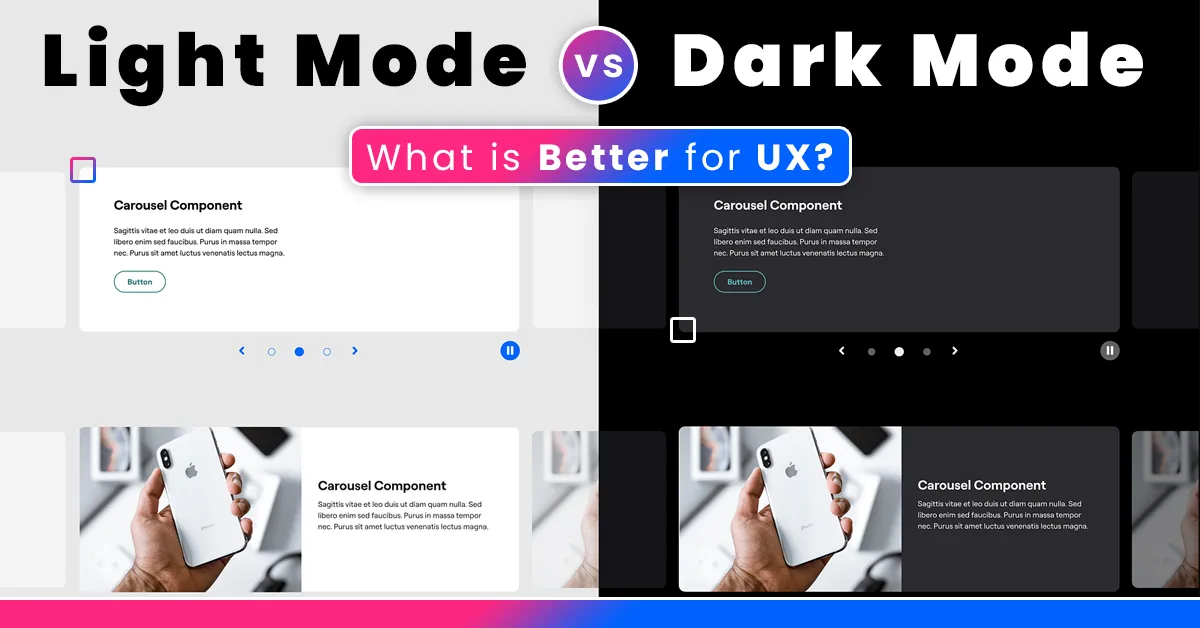
\includegraphics[width=\linewidth]{images/darkmode}
    \caption{White and dark mode comparison.~\cite{darkMode}}
    \label{fig:Darkmode}
\end{figure}


\subsection{Class aptent taciti}

\lipsum[6-7]

\begin{enumerate}
    \item Ut enim ad minim veniam, quis nostrud
    \item Ut enim ad minim 
    \item Ut enim ad minim veniam, quis 
    \begin{enumerate}
        \item Ut enim ad
        \item Ut enim ad
        \begin{enumerate}
            \item Ut enim 
            \item Ut enim 
            \begin{enumerate}
            \item Ut enim 
            \item Ut enim 
        \end{enumerate}
        \end{enumerate}
    \end{enumerate}
\end{enumerate}



\section{Testování}


Ut enim ad minim veniam, quis nostrud exercitation ullamco laboris nisi ut aliquip ex ea commodo consequat. Nulla non arcu lacinia neque faucibus fringilla. Vestibulum erat nulla, ullamcorper nec, rutrum non, nonummy ac, erat. Aliquam erat volutpat. Proin pede metus, vulputate nec, fermentum fringilla, vehicula vitae, justo.\footnote{Ut enim ad minim veniam, quis nostrud exercitation.} Etiam dictum tincidunt diam. In laoreet, magna id viverra tincidunt, sem odio bibendum justo, vel imperdiet sapien wisi sed libero. Nulla est. Maecenas fermentum, sem in pharetra pellentesque, velit turpis volutpat ante, in pharetra metus odio a lectus. Duis aute irure dolor in reprehenderit in voluptate velit esse cillum dolore eu fugiat nulla pariatur. 

\begin{lstlisting}[caption={Zbytečný kód},label=list:8-6,captionpos=b,float,abovecaptionskip=-\medskipamount,abovecaptionskip=\medskipamount,language=C]
    #include<stdio.h>
    #include<iostream>
    // A comment
    int main(void)
    {
        printf("Hello World\n");
        return 0;
    }
\end{lstlisting}

%%%%%%%%%%%%%%%%%%%%%%%%%%%%%%%%%
% alternative using package minted for source highlighting
% package minted requires execution with `-shell-escape'
% e.g., `xelatex -shell-escape ctufit-thesis.tex'
% \begin{listing}
% \begin{minted}{C}
%     #include<stdio.h>
%     #include<iostream>
%     // A comment
%     int main(void)
%     {
%         printf("Hello World\n");
%         return 0;
%     }
% \end{minted}
% \caption{Zbytečný kód}\label{list:8-6}
% \end{listing}
% %%%%%%%%%%%%%%%%%%%%%%%%%%%%%%%%%
Nullam feugiat, turpis at pulvinar vulputate, erat libero tristique tellus, nec bibendum odio risus sit amet ante. Aenean id metus id velit ullamcorper pulvinar. Fusce wisi. Integer lacinia. Aliquam id dolor. Pellentesque pretium lectus id turpis. Suspendisse sagittis ultrices augue. In laoreet, magna id viverra tincidunt, sem odio bibendum justo, vel imperdiet sapien wisi sed libero. Sed ac dolor sit amet purus malesuada congue.~\cite{Crochemore2002}

Class aptent taciti sociosqu ad litora torquent per conubia nostra, per inceptos hymenaeos. Fusce suscipit libero eget elit. Etiam dui sem, fermentum vitae, sagittis id, malesuada in, quam. Aliquam id dolor. Curabitur bibendum justo non orci. Duis viverra diam non justo. Curabitur ligula sapien, pulvinar a vestibulum quis, facilisis vel sapien. Duis condimentum augue id magna semper rutrum. Aliquam ornare wisi eu metus. Fusce aliquam vestibulum ipsum. Vivamus ac leo pretium faucibus.~\cite{Motwani2014}


\subsection{Ut enim ad minim veniam, quis nostrud}

Ut enim ad minim veniam, quis nostrud exercitation ullamco laboris nisi ut aliquip ex ea commodo consequat. Nulla non arcu lacinia neque faucibus fringilla. Vestibulum erat nulla, ullamcorper nec, rutrum non, nonummy ac, erat. Aliquam erat volutpat. Proin pede metus, vulputate nec, fermentum fringilla, vehicula vitae, justo. Etiam dictum tincidunt diam. In laoreet, magna id viverra tincidunt, sem odio bibendum justo.~\cite{Sestakova2018} 

\begin{table}\centering
\begin{tabular}{l|l|c|c}
	Typ		& Prostředí		& \LaTeX{}ovská zkratka	& \TeX{}ovská zkratka	\tabularnewline \hline 
 	Text		& \verb|math|		& \verb|\(...\)|	& \verb|$...$|	\tabularnewline \hline
 	Displayed	& \verb|displaymath|	& \verb|\[...\]|	& \verb|$$...$$|	\tabularnewline 
\end{tabular}
\caption[Příklad tabulky]{Zadávání matematiky}
\label{tab:matematika}
\end{table}


Nulla est. Maecenas fermentum, sem in pharetra pellentesque, velit turpis volutpat ante, in pharetra metus odio a lectus. Duis aute irure dolor in reprehenderit in voluptate velit esse cillum dolore eu fugiat nulla pariatur. Nullam feugiat, turpis at pulvinar vulputate, erat libero tristique tellus, nec bibendum odio risus sit amet ante. Aenean id metus id velit ullamcorper pulvinar. 

\subsubsection{Class aptent taciti}

\begin{definition}[Optional label]
Class aptent taciti sociosqu ad litora torquent per conubia nostra, per inceptos hymenaeos. Fusce suscipit libero eget elit. Etiam dui sem, fermentum vitae, sagittis id, malesuada in, quam. Aliquam id dolor. Curabitur bibendum justo non orci.
\end{definition}

\begin{example}
Class aptent taciti sociosqu ad litora torquent per conubia nostra, per inceptos hymenaeos. Fusce suscipit libero eget elit. Etiam dui sem, fermentum vitae, sagittis id, malesuada in, quam. Aliquam id dolor. Curabitur bibendum justo non orci.
\end{example}

\paragraph{Nadpis 5. úrovně}

\begin{theorem}
Class aptent taciti sociosqu ad litora torquent per conubia nostra, per inceptos hymenaeos. Fusce suscipit libero eget elit. Etiam dui sem, fermentum vitae, sagittis id, malesuada in, quam. Aliquam id dolor. Curabitur bibendum justo non orci.
\end{theorem}

\begin{proof}
Fusce suscipit libero eget elit. Etiam dui sem, fermentum vitae, sagittis id, malesuada in, quam. Aliquam id dolor. Curabitur bibendum justo non orci.
\end{proof}

\paragraph{Level 5 heading}

\begin{corollary}
Fusce suscipit libero eget elit. Etiam dui sem, fermentum vitae, sagittis id, malesuada in, quam. Aliquam id dolor. Curabitur bibendum justo non orci.
\end{corollary}

\begin{proposition}
Fusce suscipit libero eget elit. Etiam dui sem, fermentum vitae, sagittis id, malesuada in, quam. Aliquam id dolor. Curabitur bibendum justo non orci.
\end{proposition}

\begin{note}
Fusce suscipit libero eget elit. Etiam dui sem, fermentum vitae, sagittis id, malesuada in, quam. Aliquam id dolor. Curabitur bibendum justo non orci.
\end{note}

\begin{remark}
Fusce suscipit libero eget elit. Etiam dui sem, fermentum vitae, sagittis id, malesuada in, quam. Aliquam id dolor. Curabitur bibendum justo non orci.
\end{remark}

\begin{lemma}
Class aptent taciti sociosqu ad litora torquent per conubia nostra, per inceptos hymenaeos. Fusce suscipit libero eget elit. Etiam dui sem, fermentum vitae, sagittis id, malesuada in, quam. Aliquam id dolor. Curabitur bibendum justo non orci.
\end{lemma}

\lipsum[1-2]

% \subsection{Class aptent taciti sociosqu}
% 
% \lipsum[4-5]

\section{}

%---------------------------------------------------------------
\chapter{Návrh}
%---------------------------------------------------------------

V této kapitole je popsán návrh aplikace. Popíšeme architekturu celé aplikace, poté také jednotlivé komponenty, jak a k čemu slouží. Dále jsou tu také uvedeny technologie, které pro tento projekt byly zvoleny.

\section{Technologie}

V této sekci jsou probrány vybrané technologie a jejich alternativy. Je zde zdůvodněn výběr konkrétních knihoven a proč byly zvoleny namísto dostupných alternativ. Z byly zmíněny pouze knihovny, nad kterými jsem silně uvažoval při implementaci.

\subsection{Použité technologie}

Technologie v této sekci byly použity pro implementaci knihovny. Jsou zde zdůvodněny hlavní důvody pro použití a jejich popis.

\subsubsection{Robot Framework}

\subsubsection{Python}

\subsubsection{Openpyxl}

Knihovna pro zpracování dat v jazyce Python, navržená specificky pro práci s ekosystémem Office Open XML (.xlsx, .xlsm). Zjednodušuje vytváření, úpravy a parsování tabulkových souborů pomocí vysokoúrovňového python rozhraní. Abstrahuje složité vnitřní XML\footnote{Extensible Markup Language} struktury a poskytuje podporu pro mnoho operací s tabulkami, jakožto extrakci surových dat, formátování, stylování, manipulace se vzorci.

Důležité pro tento projekt je možnost použití optimalizované streamovací architektury, která umožňuje pracovat s obrovskými soubory s konstatní pamětí v read-only režimu. Spotřeba paměti může být naopak vyšší u zpracování v klasickém módu, kdy je celý soubor načten jakožto DOM\footnote{Document Object Model} do operační paměti. Jelikož je psána v pythonu, výkon je nižší než u knihoven psaných v kompilovaných jazycích, jako například \ref{sec:calamine}

\subsubsection{Xlrd}

\subsubsection{Csv module - python}

\subsubsection{Pytest}

\subsection{Nepoužité alternativy}

Zmíněné technologie v této sekci nebyly použity v projektu, ale byly uvažovány při návrhu aplikace.

\subsubsection{Pyexcel}

Zdánlivě idealní volba, knihovna, která podporuje více fomátů (.xslx, .xls, .ods, .csv, ...). Knihovna má však několik problémů, kvuli kterým nakonec nebyla využita.

Prvním problémem je memory management. I když knihovna nabízí streaming pomocí iterátorů, zpočátku je celý XML soubor, který reprezentuje jednotlivé excel soubory, naparsován do paměti najendou. Tomu jsem se chtěl v mojí knihovně vyhnout.

Dalším problémem je, že knihovna je pouze generický wrapper nad nízkoúrovňovějšími knihovnami, není to engine. Použitím knihovny akorát ztrácíme kontrolu nad informacemi z knihoven, které tato knihovna používá.

V poslední řadě také omezené operace a datové typy, které knihovna podporuje. Pro .xlsx není podporováno formátování ani makra, jelikož knihovna je čistě datová. V této práci se sice také zaměřuji čistě na data, ale potenciálně v budoucnu je tam možnost přidat i tyto možnosti. Chybí kontrola nad vrácenými datovými typy, kdy nevíme, jak je s daty na pozadí naloženo a jak se transformují.\cite{Pyexcel}

\subsubsection{Python-calamine} \label{sec:calamine}

Knihovna napsaná v rustu, která má pouze python wrapper. Tím, že je napsána v rustu, je násobně rychlejší než její konkurenti, kteří jsou napsáni v čistém pythonu. Také podporuje formáty .xlsx, .xls, .ods. Je také paměťově úsporná, nenačítá celý soubor do paměti.

Tato knihovna ovšem také nakonec použita nebyla. Knihovna je read-only, což znamená znemožnění psaní do načtených souborů. Dále je nutnost mít nainstalován rust. Jelikož automatické testy jsou často spostěny v github-actions, je nutnost mít nainstalovaný rust, což je pouze kvůli testům nevyžadující. Tím, že je knihovna optimalizovaná na výkon, extrahuje pouze čisté hodnoty, tím ztrácíme jakékoliv další informace, které pomocí jiných knihoven jsme schopni získat.

I přes všechny nevýhody zmíněné výše se dá do budoucna uvažovat o použití této knihovny v režimu streamování díky vysoké rychlosti a paměťové úspornosti. \cite{Python-calamine}

\subsubsection{Xlwt}

Knihovna pro zapisování do souborů v .xls formátu. Jelikož tento projekt se zaměřuje hlavně na testování, knihovna nakonec nebyla použita. Zápis do starých souborů v aplikaci už nedává smysl. Zároveň knihovna již není dále vyvíjena, pouze udržována, podle autora už nemá být používána, pokud není vysloveně nutno.\cite{xlwtEnd} \cite{xlwt}

\subsubsection{Pandas}

Knihovna používána hlavně in-memory datavou analýzu. Hlavním problémem je nutnost načíst celý soubor do DF\footnote{DataFrame}. Sice je možné práci s většími soubory trochu zeefktivnit z ohledu paměti, ale pro tento projekt jsem se rozhodl tyto metody neimplementovat.\cite{PandasScale} \cite{Pandas}

\section{Donec odio tempus molestie}

\lipsum[2]~\cite{def:1, def:2}

\subsection{Class aptent taciti}

\lipsum[2-3]

\begin{description}
\item[Kapitola 1] Lorem ipsum dolor sit amet, consectetuer adipiscing elit. Curabitur sagittis hendrerit ante. Class aptent taciti sociosqu ad litora tor\-quent per conubia nostra, per inceptos hymenaeos. Cras pede libero, dapibus nec, pretium sit amet, tempor quis.

\item[Kapitola 2] Lorem ipsum dolor sit amet, consectetuer adipiscing elit. Curabitur sagittis hendrerit ante. Class aptent taciti sociosqu ad litora tor\-quent per conubia nostra, per inceptos hymenaeos. Cras pede libero, dapibus nec, pretium sit amet, tempor quis.

\item[Kapitola 3] Lorem ipsum dolor sit amet, consectetuer adipiscing elit. Curabitur sagittis hendrerit ante. Class aptent taciti sociosqu ad litora tor\-quent per conubia nostra, per inceptos hymenaeos. Cras pede libero, dapibus nec, pretium sit amet, tempor quis.

\item[Kapitola 4] Lorem ipsum dolor sit amet, consectetuer adipiscing elit. Curabitur sagittis hendrerit ante. Class aptent taciti sociosqu ad litora tor\-quent per conubia nostra, per inceptos hymenaeos. Cras pede libero, dapibus nec, pretium sit amet, tempor quis.~\cite{jakZiskatAcko}
\end{description}

\lipsum[2]

\section{Lorem ipsum dolor sit amet}

\lipsum[3-5]

\chapter{Implementace}

\section{Testování}

\section{Nasazení}

\chapter{Závěr}
